\documentclass[aspectratio=169]{beamer}

%------------------------------------------------
% Packages & Fonts
%------------------------------------------------
\usepackage[utf8]{inputenc}
\usepackage{graphicx}
\usepackage{xcolor}
\usepackage{tikz}
\usepackage{lmodern}
\usepackage{amsmath}
\usepackage{booktabs}
\usepackage{multirow}
\usepackage{appendixnumberbeamer}
\graphicspath{{Figures/}{/home/sares/Documents/HGV2/figures/validation_final_rbf363_v2/}{/home/sares/Documents/HGV2/figures/}{/home/sares/Documents/HGV2/figures/validation_final_rbf363/}{/home/sares/Documents/HGV2/figures/validation_final_rbf363/error_maps/}{/home/sares/Documents/HGV2/figures/validation_final_rbf363/coefficients/}}

%------------------------------------------------
% Stanford Colors
%------------------------------------------------
\definecolor{stanfordred}{HTML}{8C1515}
\definecolor{customlightgray}{rgb}{0.9,0.9,0.9}

%------------------------------------------------
% Theme & Color Overrides
%------------------------------------------------
\usetheme{Dresden}

\setbeamercolor{structure}{fg=stanfordred}
\setbeamercolor{title}{fg=stanfordred}
\setbeamercolor{frametitle}{bg=stanfordred, fg=white}
\setbeamercolor{itemize item}{fg=stanfordred}
\setbeamercolor{section in toc}{fg=stanfordred}
\setbeamertemplate{caption}[numbered]

\setbeamercolor{section in head/foot}{bg=customlightgray, fg=stanfordred}
\setbeamerfont{section in head/foot}{size=\scriptsize}
\setbeamertemplate{navigation symbols}{}

%------------------------------------------------
% Custom Footline: only frame number
%------------------------------------------------
\setbeamertemplate{footline}{%
  \leavevmode%
  \hbox{%
    \hspace*{0.85\paperwidth}%
    \begin{beamercolorbox}[wd=0.15\paperwidth,ht=2.5ex,dp=1ex,right]{date in head/foot}%
      \insertframenumber{} / \inserttotalframenumber%
    \end{beamercolorbox}%
  }%
}

\setbeamerfont{frametitle}{size=\small}

%------------------------------------------------
% Document Info
%------------------------------------------------
\title{Global and Local Projection-Based Reduced-Order Models}
\subtitle{2D Burgers and Hypersonic Vehicle Campaigns}

\author{%
Sebastian Ares de Parga\textsuperscript{1}, \
Radek Tezaur\textsuperscript{1}, \
Charbel Farhat\textsuperscript{1,2} \
}

\institute{%
  \inst{1} Department of Aeronautics and Astronautics\\
  \inst{2} Institute for Computational and Mathematical Engineering\\
  Stanford University, Stanford, CA 94305, USA\\[0.5ex]
}

\date{\today}

\begin{document}

\begin{frame}
  \titlepage
\end{frame}

\section{2D Burgers Campaign}

\begin{frame}{2D Burgers Campaign}
\centering
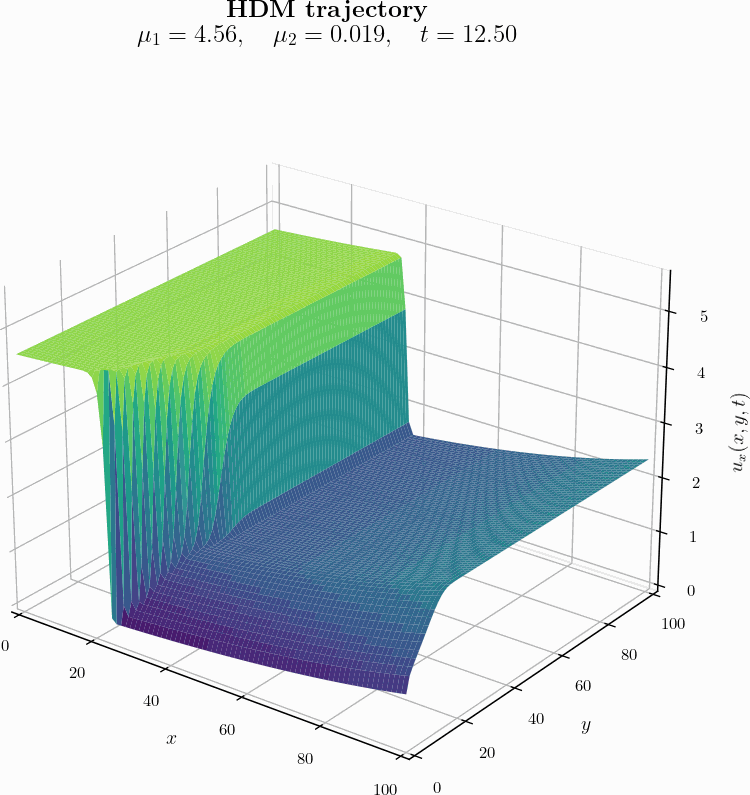
\includegraphics[height=0.56\textheight,keepaspectratio]{Figures/burgers_hdm_3d_transition_cropped.png}\\[0.20cm]
\Large Global and local HPROM validation\\[0.12cm]
\normalsize Linear POD bases, quadratic manifolds, and GPR manifolds
\end{frame}

\begin{frame}{Parameter Domain and Test Points}
\centering
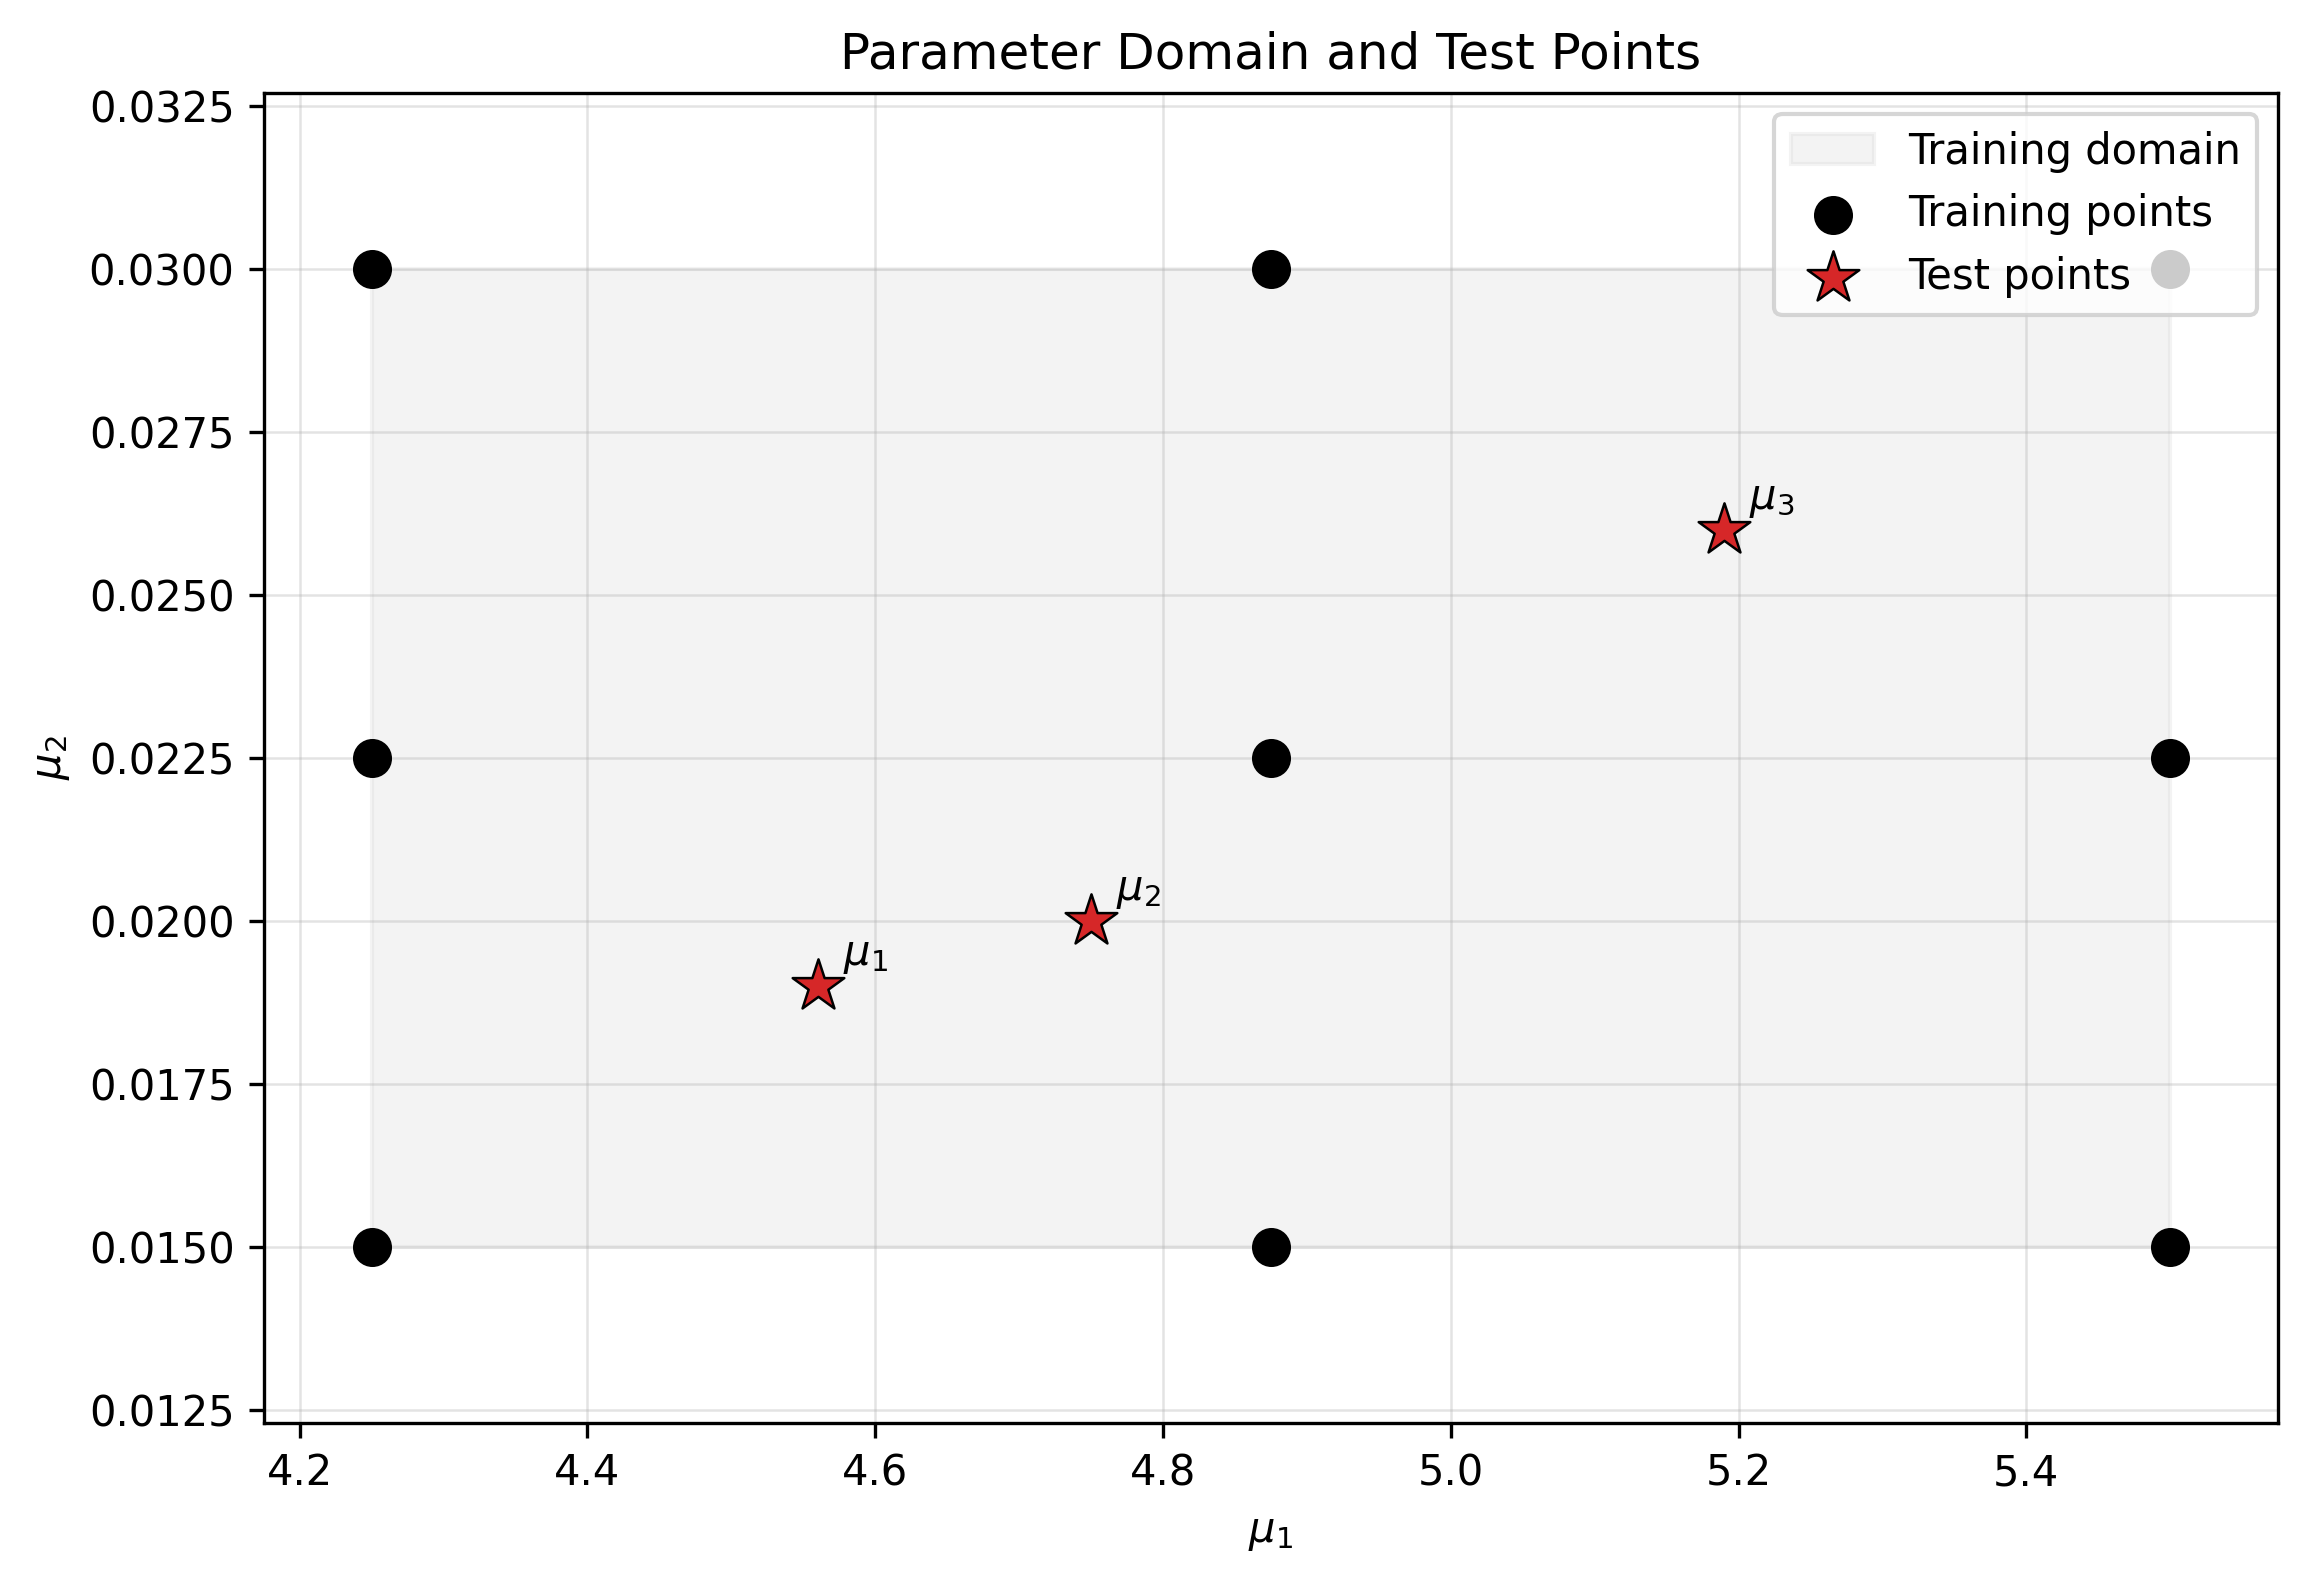
\includegraphics[width=0.82\textwidth,height=0.70\textheight,keepaspectratio]{Figures/parameter_domain_and_test_points.png}
\end{frame}

\newcommand{\BurgersTheoryFrames}{%
\begin{frame}{Global ROM Storyline: LSPG + Gauss-Newton}
\small
Given the implicit HDM residual $\mathbf{r}(\mathbf{u})=\mathbf{0}$, define a manifold
\[
\mathbf{u}\approx \mathbf{u}_{\mathrm{ref}}+\widetilde{\mathbf{u}}(\mathbf{q}).
\]
LSPG solves at each time step:
\[
\mathbf{q}^{\star}
=\arg\min_{\mathbf{q}}\;
\frac{1}{2}\left\|\mathbf{r}\!\left(\mathbf{u}_{\mathrm{ref}}+\widetilde{\mathbf{u}}(\mathbf{q})\right)\right\|_2^2.
\]
With Gauss-Newton (current iterate $\mathbf{q}^{(k)}$), the increment $\Delta\mathbf{q}$ is obtained from
\[
\left(\mathbf{\Psi}^{T}\mathbf{J}^{T}\mathbf{J}\mathbf{\Psi}\right)\Delta\mathbf{q}
=-\mathbf{\Psi}^{T}\mathbf{J}^{T}\mathbf{r},
\]
where
\[
\mathbf{\Psi}=\frac{\partial\widetilde{\mathbf{u}}}{\partial\mathbf{q}},
\qquad
\mathbf{J}=\frac{\partial\mathbf{r}}{\partial\mathbf{u}},
\qquad
\mathbf{q}^{(k+1)}=\mathbf{q}^{(k)}+\Delta\mathbf{q}.
\]
\end{frame}

\begin{frame}{Global Linear HPROM}
\small
State ansatz:
\[
\mathbf{u}\approx \mathbf{u}_{\mathrm{ref}}+\mathbf{V}\mathbf{q},
\qquad
\mathbf{V}\in\mathbb{R}^{N\times n},\; n=96.
\]
Hence
\[
\widetilde{\mathbf{u}}(\mathbf{q})=\mathbf{V}\mathbf{q},
\qquad
\mathbf{\Psi}=\frac{\partial\widetilde{\mathbf{u}}}{\partial\mathbf{q}}=\mathbf{V}.
\]
Gauss-Newton system:
\[
\left(\mathbf{V}^{T}\mathbf{J}^{T}\mathbf{J}\mathbf{V}\right)\Delta\mathbf{q}
=-\mathbf{V}^{T}\mathbf{J}^{T}\mathbf{r}.
\]
\end{frame}

\begin{frame}{Global HQPROM}
\small
Quadratic-manifold ansatz:
\[
\mathbf{u}\approx
\mathbf{u}_{\mathrm{ref}}
+\mathbf{V}\mathbf{q}
+\mathbf{H}\left(\mathbf{q}\otimes\mathbf{q}\right),
\qquad
n=39.
\]
Thus
\[
\widetilde{\mathbf{u}}(\mathbf{q})
=\mathbf{V}\mathbf{q}
+\mathbf{H}\left(\mathbf{q}\otimes\mathbf{q}\right),
\]
and the tangent depends on the current reduced state:
\[
\mathbf{\Psi}(\mathbf{q})
=\frac{\partial\widetilde{\mathbf{u}}}{\partial\mathbf{q}}
=\mathbf{V}
+\frac{\partial}{\partial\mathbf{q}}
\!\left[\mathbf{H}\left(\mathbf{q}\otimes\mathbf{q}\right)\right].
\]
\end{frame}

\begin{frame}{Global HPROM-GPR}
\small
Split basis and reduced coordinates:
\[
\mathbf{V}_{\mathrm{tot}}=[\mathbf{V},\bar{\mathbf{V}}],
\qquad
\mathbf{q}_{\mathrm{tot}}=
\begin{bmatrix}
\mathbf{q}\\
\bar{\mathbf{q}}
\end{bmatrix}.
\]
\[
\bar{\mathbf{q}}=\mathcal{N}_{\mathrm{GPR}}(\mathbf{q}),
\qquad
n=20,\;\bar{n}=131.
\]
State ansatz:
\[
\mathbf{u}\approx
\mathbf{u}_{\mathrm{ref}}
+\widetilde{\mathbf{u}}(\mathbf{q}),
\]
\[
\widetilde{\mathbf{u}}(\mathbf{q})
=\mathbf{V}_{\mathrm{tot}}\mathbf{q}_{\mathrm{tot}}
=\mathbf{V}\mathbf{q}
+\bar{\mathbf{V}}\,\mathcal{N}_{\mathrm{GPR}}(\mathbf{q}).
\]
Effective tangent for Gauss-Newton:
\[
\mathbf{\Psi}(\mathbf{q})
=\frac{\partial\widetilde{\mathbf{u}}}{\partial\mathbf{q}}
=\mathbf{V}
+\bar{\mathbf{V}}\frac{\partial\mathcal{N}_{\mathrm{GPR}}}{\partial\mathbf{q}}.
\]
\end{frame}

\begin{frame}{Local ROMs: Piecewise Manifolds}
\small
Partition the training snapshots into clusters $k=1,\dots,N_c$ and build one local trial manifold per cluster:
\[
\mathbf u \approx \Phi_k(\mathbf q_k).
\]

Examples used in this work:
\[
\Phi_k^{\mathrm{lin}}(\mathbf q)
=
\mathbf u_{0,k}+\mathbf V_k\mathbf q,
\]
\[
\Phi_k^{\mathrm{quad}}(\mathbf q)
=
\mathbf u_{0,k}+\mathbf V_k\mathbf q+\mathbf H_k(\mathbf q\otimes\mathbf q),
\]
\[
\Phi_k^{\mathrm{gpr}}(\mathbf q)
=
\mathbf u_{0,k}+\mathbf V_k\mathbf q+\bar{\mathbf V}_k\,\mathcal N_{\mathrm{GPR},k}(\mathbf q).
\]

\vspace{0.3em}
\textbf{Online workflow}
\begin{enumerate}
\item Select the active cluster.
\item If the cluster changes, transfer the current state to the new local manifold.
\item Solve the local LSPG problem in the active manifold.
\end{enumerate}
\end{frame}

\begin{frame}{Cluster Selection: Final Form (Linear)}
\small
Shared nearest-centroid selector (used in all local models):
\[
k^+=\arg\min_{\ell=1,\dots,N_c}\|\mathbf u^s-\mathbf u_{c,\ell}\|_2^2,
\qquad
\mathbf u^s=\Phi_{k^-}(\mathbf q_{k^-}).
\]

\vspace{0.2em}
For the linear local manifold $\Phi_{k^-}^{\mathrm{lin}}(\mathbf q)=\mathbf u_{0,k^-}+\mathbf V_{k^-}\mathbf q$:
\[
k^+=\arg\min_{\ell=1,\dots,N_c} S_{k^-,\ell}^{\mathrm{lin}}(\mathbf q_{k^-}),
\]
\[
S_{k^-,\ell}^{\mathrm{lin}}(\mathbf q)
=
2\,\mathbf g_{k^-,\ell}^T\mathbf q + d_{k^-,\ell},
\]
with offline-precomputed terms
\[
\mathbf g_{k^-,\ell}
:=
\mathbf V_{k^-}^T(\mathbf u_{0,k^-}-\mathbf u_{c,\ell}),
\qquad
d_{k^-,\ell}
:=
\|\mathbf u_{0,k^-}-\mathbf u_{c,\ell}\|_2^2.
\]
\end{frame}

\begin{frame}{Cluster Selection: Final Form (HQPROM and HPROM-GPR)}
\scriptsize
\textbf{HQPROM selector}
\[
k^+=\arg\min_{\ell} S_{k^-,\ell}^{\mathrm{quad}}(\mathbf q_{k^-}),
\]
\[
S_{k^-,\ell}^{\mathrm{quad}}(\mathbf q)
=
2\,\mathbf g_{k^-,\ell}^T\mathbf q
+
2\,\mathbf m_{k^-,\ell}^T(\mathbf q\otimes\mathbf q)
+
d_{k^-,\ell},
\]
\[
\mathbf m_{k^-,\ell}^T(\mathbf q\otimes\mathbf q)
:=
(\mathbf u_{0,k^-}-\mathbf u_{c,\ell})^T\mathbf H_{k^-}(\mathbf q\otimes\mathbf q).
\]

\vspace{0.35em}
\textbf{HPROM-GPR selector}
\[
k^+=\arg\min_{\ell} S_{k^-,\ell}^{\mathrm{gpr}}(\mathbf q_{k^-}),
\]
\[
S_{k^-,\ell}^{\mathrm{gpr}}(\mathbf q)
=
2\,\mathbf g_{k^-,\ell}^T\mathbf q
+
2\,\bar{\mathbf g}_{k^-,\ell}^T\mathcal N_{\mathrm{GPR},k^-}(\mathbf q)
+
d_{k^-,\ell}.
\]
\[
\bar{\mathbf q}_{k^-}:=\mathcal N_{\mathrm{GPR},k^-}(\mathbf q_{k^-}),
\qquad
\bar{\mathbf g}_{k^-,\ell}:=\bar{\mathbf V}_{k^-}^T(\mathbf u_{0,k^-}-\mathbf u_{c,\ell}).
\]
\end{frame}

\begin{frame}{Cluster Change: Linear and Nonlinear Transfers}
\scriptsize
\[
k^+=k^- \Rightarrow \text{no transfer},
\qquad
k^+\neq k^- \Rightarrow \text{solve transfer problem}.
\]
Transferred state:
\[
\mathbf u^s=\Phi_{k^-}(\mathbf q_{k^-}).
\]

\textbf{Linear local target}
\[
\mathbf q_{k^+}^{\mathrm{lin}}
=\arg\min_{\mathbf q}
\left\|
\mathbf u^s-\left(\mathbf u_{0,k^+}+\mathbf V_{k^+}\mathbf q\right)
\right\|_2^2,
\]
\[
\text{if }\mathbf V_{k^+}^T\mathbf V_{k^+}=\mathbf I,\quad
\mathbf q_{k^+}^{\mathrm{lin}}=\mathbf V_{k^+}^T(\mathbf u^s-\mathbf u_{0,k^+}).
\]

\textbf{Nonlinear local targets (HQPROM / HPROM-GPR)}
\[
\mathbf q_{k^+}^{\mathrm{nl}}
=\arg\min_{\mathbf q}
\left\|\mathbf u^s-\Phi_{k^+}^{\mathrm{nl}}(\mathbf q)\right\|_2^2.
\]
\end{frame}

\begin{frame}{Cluster Change: Nonlinear Least Squares}
\small
For nonlinear local manifolds, define
\[
\mathbf r_{\mathrm{tr}}(\mathbf q):=\Phi_{k^+}(\mathbf q)-\mathbf u^s,
\qquad
\mathbf J_{\Phi}(\mathbf q):=\frac{\partial \Phi_{k^+}}{\partial \mathbf q}.
\]
Gauss--Newton at iterate $\mathbf q^{(j)}$:
\[
\left(\mathbf J_{\Phi}^T\mathbf J_{\Phi}\right)\Delta\mathbf q
=
-\mathbf J_{\Phi}^T\mathbf r_{\mathrm{tr}}(\mathbf q^{(j)}),
\qquad
\mathbf q^{(j+1)}=\mathbf q^{(j)}+\Delta\mathbf q.
\]
\end{frame}

}

\begin{frame}{Online Performance ($250\times250$): Avg/Max Error over 3 Test Points}
\scriptsize
\centering
\resizebox{\textwidth}{!}{%
\begin{tabular}{lrrrrrrr}
\hline
\textbf{Computational model} & $n$ ($N$ for HDM) & $\bar{n}$ & $N_e$ & avg $\mathbb{RE}_{2,\mathbf{u}}$ (\%) & max $\mathbb{RE}_{2,\mathbf{u}}$ (\%) & Wall-clock time (min) & Speedup \\
\hline
HDM & 125\,000 & -- & 62\,500 & -- & -- & 12.517 & -- \\
\addlinespace[0.35em]
HPROM & 96 & -- & 4\,241 & 1.030 & 1.096 & 0.366 & 34.2 \\
HQPROM & 39 & -- & 3\,460 & 0.818 & 0.861 & 0.641 & 19.5 \\
HPROM-GPR & 20 & 131 & 1\,799 & 0.666 & 0.785 & 0.236 & 53.1 \\
\addlinespace[0.35em]
Local HPROM ($N_c=3$) & 35--48 & -- & 3\,405 & 0.897 & 0.933 & 0.154 & 81.4 \\
Local HQPROM ($N_c=3$) & 21--27 & -- & 2\,152 & 0.888 & 1.025 & 0.215 & 58.3 \\
Local HPROM-GPR ($N_c=3$) & 9 & 60--97 & 811 & 0.714 & 0.786 & 0.113 & 110.5 \\
\addlinespace[0.35em]
Local HPROM ($N_c=5$) & 23--31 & -- & 2\,384 & 0.915 & 0.943 & 0.095 & 132.0 \\
Local HQPROM ($N_c=5$) & 15--20 & -- & 1\,593 & 0.760 & 0.878 & 0.128 & 97.9 \\
Local HPROM-GPR ($N_c=5$) & 7 & 41--68 & 631 & 0.673 & 0.880 & 0.094 & 133.2 \\
\hline
\end{tabular}}
\vspace{0.2em}

{\tiny Speedup is computed with respect to the HDM runtime, $t_{\mathrm{HDM}}=751.043$ s, averaged over the three test points.}

{\tiny Online timings were measured on Sherlock using one node, 24 MPI ranks, and 24 cores.}

{\tiny $N_e$ denotes the number of sampled ECSW elements ($N_e=62{,}500$ for HDM/full mesh).}

{\tiny All models are reported at a matched accuracy target of $1\% \pm 0.2\%$ in max $\mathbb{RE}_{2,\mathbf{u}}$: for each $N_c$ the accuracy knob is tuned into that window ($\mathtt{pod\_tol}$ for Local HPROM, $\zeta_{\mathrm{qua}}$ for Local HQPROM, $n$ for Local HPROM-GPR), so differences in $n$, $N_e$ and speedup are read at constant accuracy.}
\end{frame}

\begin{frame}{Global Reduced Meshes (ECSW)}
\centering
\begin{columns}[T]
\column{0.33\textwidth}
\centering

\includegraphics[width=\linewidth]{hprom_reduced_mesh.png}\\
{\tiny HPROM ($N_e=4{,}241$)}

\column{0.33\textwidth}
\centering

\includegraphics[width=\linewidth]{hqprom_reduced_mesh.png}\\
{\tiny HQPROM ($N_e=3{,}460$)}

\column{0.33\textwidth}
\centering

\includegraphics[width=\linewidth]{hprom_gpr_reduced_mesh.png}\\
{\tiny HPROM-GPR ($N_e=1{,}799$)}
\end{columns}
\end{frame}

\begin{frame}{Local Reduced Meshes (ECSW), $N_c=3$}
\centering
\begin{columns}[T]
\column{0.33\textwidth}
\centering

\includegraphics[width=\linewidth]{local_hprom_reduced_mesh.png}\\
{\tiny Local HPROM ($N_e=3{,}405$)}

\column{0.33\textwidth}
\centering

\includegraphics[width=\linewidth]{local_hqprom_reduced_mesh.png}\\
{\tiny Local HQPROM ($N_e=2{,}152$)}

\column{0.33\textwidth}
\centering

\includegraphics[width=\linewidth]{local_hprom_gpr_reduced_mesh.png}\\
{\tiny Local HPROM-GPR ($N_e=811$)}
\end{columns}
\end{frame}

\begin{frame}{Burgers Conclusions}
\small
\begin{itemize}
  \item At matched accuracy, every local ROM is faster than its global counterpart:
        $34.2\times\!\to\!132.0\times$ (HPROM), $19.5\times\!\to\!97.9\times$ (HQPROM),
        $53.1\times\!\to\!133.2\times$ (HPROM--GPR).
  \item Within each family the speedup grows monotonically with $N_c$, so clustering is
        the dominant lever rather than the choice of local manifold.
  \item When the nonlinear manifold does not compress enough, as for the quadratic, the
        speedup reached at a given error need not beat the linear model. This is
        problem-dependent, so the three families are alternatives rather than a ranking.
  \item Clustering and nonlinear compression are not additive. A linear basis always gains
        from more clusters, whereas HPROM--GPR already carries an intrinsic compression
        that clustering should support rather than replace: at $N_c=5$ the local linear
        HPROM has caught up with it ($132.0\times$ versus $133.2\times$), and raising
        $N_c$ further would make HPROM--GPR more expensive, since every nonlinear step
        also pays for the manifold tangent
        $\mathbf{\Psi}=\mathbf{V}+\bar{\mathbf{V}}\,\partial\mathcal{N}_{\mathrm{GPR}}/
        \partial\mathbf{q}$, the closure evaluation, and cluster selection and transfer.
\end{itemize}
\end{frame}

\newcommand{\BurgersSolutionFigureFrames}{%
\begin{frame}{HPROM vs HDM: $\boldsymbol\mu=(4.56,\,0.019)$}
\centering

\includegraphics[width=0.82\textwidth,height=0.70\textheight,keepaspectratio]{Figures/hprom_vs_hdm_mu1_4.56_mu2_0.019.png}
\end{frame}

\begin{frame}{HPROM vs HDM: $\boldsymbol\mu=(4.75,\,0.020)$}
\centering

\includegraphics[width=0.82\textwidth,height=0.70\textheight,keepaspectratio]{Figures/hprom_vs_hdm_mu1_4.75_mu2_0.020.png}
\end{frame}

\begin{frame}{HPROM vs HDM: $\boldsymbol\mu=(5.19,\,0.026)$}
\centering

\includegraphics[width=0.82\textwidth,height=0.70\textheight,keepaspectratio]{Figures/hprom_vs_hdm_mu1_5.19_mu2_0.026.png}
\end{frame}

\begin{frame}{Local HPROM ($N_c=3$) vs HDM: $\boldsymbol\mu=(4.56,\,0.019)$}
\centering

\includegraphics[width=0.82\textwidth,height=0.70\textheight,keepaspectratio]{Figures/local_hprom_vs_hdm_mu1_4.56_mu2_0.019.png}
\end{frame}

\begin{frame}{Local HPROM ($N_c=3$) vs HDM: $\boldsymbol\mu=(4.75,\,0.020)$}
\centering

\includegraphics[width=0.82\textwidth,height=0.70\textheight,keepaspectratio]{Figures/local_hprom_vs_hdm_mu1_4.75_mu2_0.020.png}
\end{frame}

\begin{frame}{Local HPROM ($N_c=3$) vs HDM: $\boldsymbol\mu=(5.19,\,0.026)$}
\centering

\includegraphics[width=0.82\textwidth,height=0.70\textheight,keepaspectratio]{Figures/local_hprom_vs_hdm_mu1_5.19_mu2_0.026.png}
\end{frame}

\begin{frame}{HQPROM vs HDM: $\boldsymbol\mu=(4.56,\,0.019)$}
\centering

\includegraphics[width=0.82\textwidth,height=0.70\textheight,keepaspectratio]{Figures/hqprom_vs_hdm_mu1_4.56_mu2_0.019.png}
\end{frame}

\begin{frame}{HQPROM vs HDM: $\boldsymbol\mu=(4.75,\,0.020)$}
\centering

\includegraphics[width=0.82\textwidth,height=0.70\textheight,keepaspectratio]{Figures/hqprom_vs_hdm_mu1_4.75_mu2_0.020.png}
\end{frame}

\begin{frame}{HQPROM vs HDM: $\boldsymbol\mu=(5.19,\,0.026)$}
\centering

\includegraphics[width=0.82\textwidth,height=0.70\textheight,keepaspectratio]{Figures/hqprom_vs_hdm_mu1_5.19_mu2_0.026.png}
\end{frame}

\begin{frame}{Local HQPROM ($N_c=3$) vs HDM: $\boldsymbol\mu=(4.56,\,0.019)$}
\centering

\includegraphics[width=0.82\textwidth,height=0.70\textheight,keepaspectratio]{Figures/local_hqprom_vs_hdm_mu1_4.56_mu2_0.019.png}
\end{frame}

\begin{frame}{Local HQPROM ($N_c=3$) vs HDM: $\boldsymbol\mu=(4.75,\,0.020)$}
\centering

\includegraphics[width=0.82\textwidth,height=0.70\textheight,keepaspectratio]{Figures/local_hqprom_vs_hdm_mu1_4.75_mu2_0.020.png}
\end{frame}

\begin{frame}{Local HQPROM ($N_c=3$) vs HDM: $\boldsymbol\mu=(5.19,\,0.026)$}
\centering

\includegraphics[width=0.82\textwidth,height=0.70\textheight,keepaspectratio]{Figures/local_hqprom_vs_hdm_mu1_5.19_mu2_0.026.png}
\end{frame}

\begin{frame}{HPROM-GPR vs HDM: $\boldsymbol\mu=(4.56,\,0.019)$}
\centering

\includegraphics[width=0.82\textwidth,height=0.70\textheight,keepaspectratio]{Figures/hprom_gpr_vs_hdm_mu1_4.56_mu2_0.019.png}
\end{frame}

\begin{frame}{HPROM-GPR vs HDM: $\boldsymbol\mu=(4.75,\,0.020)$}
\centering

\includegraphics[width=0.82\textwidth,height=0.70\textheight,keepaspectratio]{Figures/hprom_gpr_vs_hdm_mu1_4.75_mu2_0.020.png}
\end{frame}

\begin{frame}{HPROM-GPR vs HDM: $\boldsymbol\mu=(5.19,\,0.026)$}
\centering

\includegraphics[width=0.82\textwidth,height=0.70\textheight,keepaspectratio]{Figures/hprom_gpr_vs_hdm_mu1_5.19_mu2_0.026.png}
\end{frame}

\begin{frame}{Local HPROM-GPR ($N_c=3$) vs HDM: $\boldsymbol\mu=(4.56,\,0.019)$}
\centering

\includegraphics[width=0.82\textwidth,height=0.70\textheight,keepaspectratio]{Figures/local_hprom_gpr_vs_hdm_mu1_4.56_mu2_0.019.png}
\end{frame}

\begin{frame}{Local HPROM-GPR ($N_c=3$) vs HDM: $\boldsymbol\mu=(4.75,\,0.020)$}
\centering

\includegraphics[width=0.82\textwidth,height=0.70\textheight,keepaspectratio]{Figures/local_hprom_gpr_vs_hdm_mu1_4.75_mu2_0.020.png}
\end{frame}

\begin{frame}{Local HPROM-GPR ($N_c=3$) vs HDM: $\boldsymbol\mu=(5.19,\,0.026)$}
\centering

\includegraphics[width=0.82\textwidth,height=0.70\textheight,keepaspectratio]{Figures/local_hprom_gpr_vs_hdm_mu1_5.19_mu2_0.026.png}
\end{frame}

}

\section{Hypersonic Vehicle Campaign}

\begin{frame}{Hypersonic Vehicle Campaign}
\centering
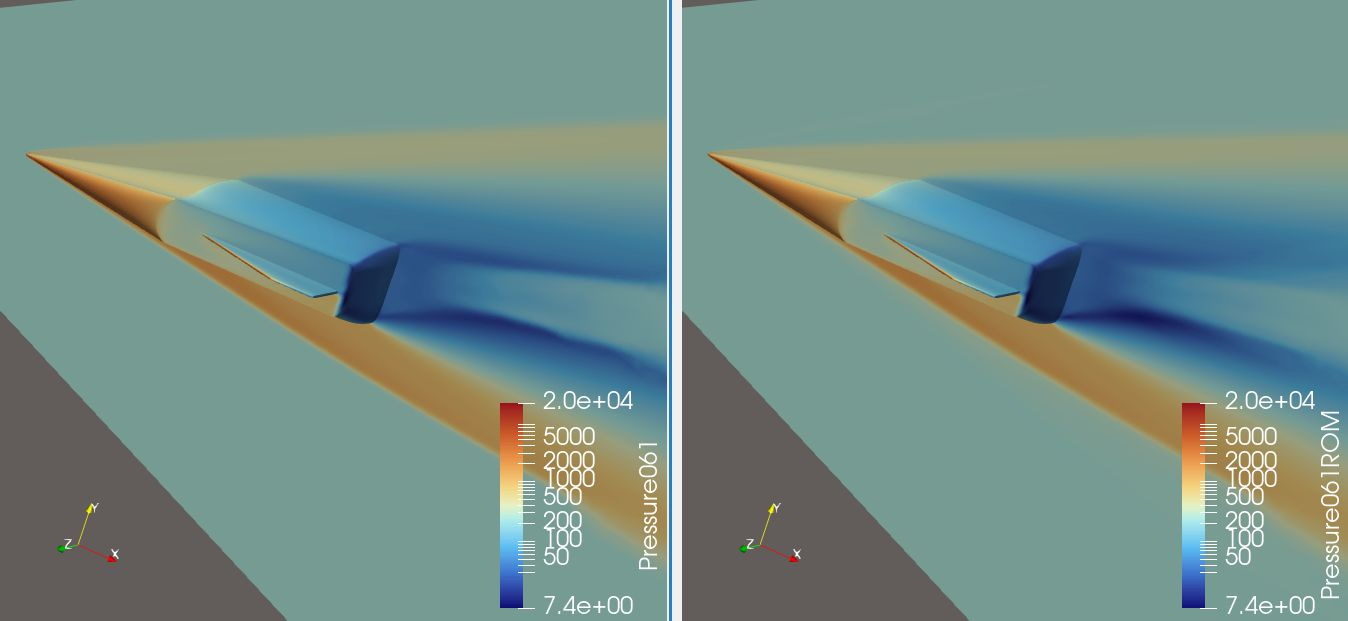
\includegraphics[width=\textwidth,height=0.59\textheight,keepaspectratio]{Figures/img38.jpg}\\[0.25cm]
\Large Global and local HPROM validation\\[0.16cm]
\normalsize Linear POD bases and RBF manifolds
\end{frame}

\begin{frame}{Training and Validation Space}
\centering
\small
363 HDM training cases; 100 independent HDM validation cases; four local clusters with 20\% overlap; ECSW tolerance $10^{-3}$.

\vspace{0.35cm}
\includegraphics[width=0.97\textwidth,height=0.64\textheight,keepaspectratio]{training_validation_space.png}
\end{frame}

\begin{frame}{HGV2 ROM Configurations}
\centering
\small
\renewcommand{\arraystretch}{1.15}
\begin{tabular}{lccc}
\hline
\textbf{Model} & \textbf{Reduction} & \textbf{Closure} & $N_c$ \\
\hline
HPROM & one POD basis & -- & 1 \\
HPROM--RBF & $n=8$ primary coordinates & one RBF map & 1 \\
\addlinespace[0.35em]
Local HPROM & one POD basis per cluster & -- & 4 \\
Local HPROM--RBF & $n=8$ primary coordinates & one RBF map per cluster & 4 \\
\hline
\end{tabular}

\vspace{0.5em}
{\small Every POD basis and RBF map is trained from the same 363 HDM parameter cases.
Each online state is assigned to its nearest cluster. ECSW is an independent offline
construction step.}
\end{frame}

\begin{frame}{HGV2 Online Performance and Validation Accuracy}
\scriptsize
\centering
\resizebox{\textwidth}{!}{%
\begin{tabular}{lrrrrrrr}
\hline
\textbf{Computational model} & $n$ ($N$ for HDM) & $\bar{n}$ & $C_D$ (\%) & $C_L$ (\%) & $C_M$ (\%) & Online time (s) & Speedup \\
\hline
HDM & 5\,674\,883 & -- & -- & -- & -- & \textit{pending} & -- \\
\addlinespace[0.35em]
HPROM & 362 & -- & 0.975 & 0.554 & 6.620 & 24.03 & -- \\
HPROM--RBF & 8 & 354 & 1.388 & 1.335 & 7.004 & 1.15 & 21.0 \\
\addlinespace[0.35em]
Local HPROM ($N_c=4$) & 95--168 & -- & 1.101 & 0.444 & 6.242 & 6.80 & 3.5 \\
Local HPROM--RBF ($N_c=4$) & 8 & 117--140 & 1.978 & 2.183 & 7.117 & 0.62 & 38.9 \\
\hline
\end{tabular}}
\vspace{0.2em}

{\tiny Coefficient errors are global relative $L^2$ values over 100 independent validation cases.}

{\tiny Speedup is computed with respect to the HPROM online time, so HPROM itself carries no entry. The HDM runtime is pending.}

{\tiny Timings are means over 10 validation cases, measured on Sherlock using one node, 24 MPI ranks, and 24 cores.}

{\tiny For the HDM, $N$ is the number of mesh nodes. For HPROM, $n$ is the full POD rank. For HPROM--RBF, $n$ and $\bar{n}$ are the primary and secondary dimensions; local $\bar{n}$ is the range across the four cluster bases.}
\end{frame}

\begin{frame}{HGV2 Validation Error Comparison}
\centering
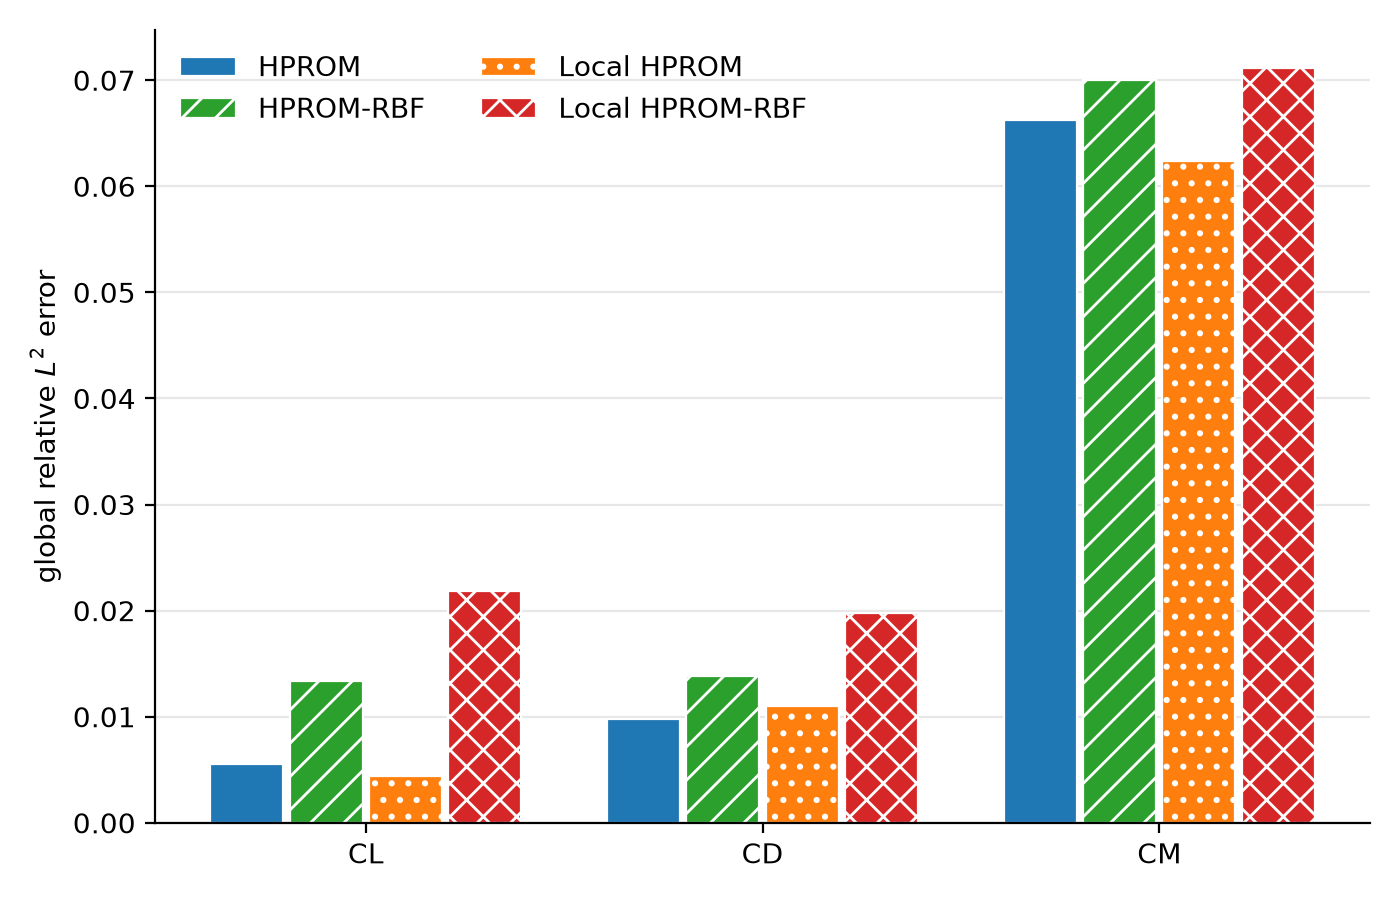
\includegraphics[width=0.91\textwidth,height=0.74\textheight,keepaspectratio]{overall_relative_errors.png}
\end{frame}

\begin{frame}{HGV2 ECSW Offline Cost}
\centering
\scriptsize
\renewcommand{\arraystretch}{1.20}
\resizebox{0.86\textwidth}{!}{%
\begin{tabular}{lrrr}
\hline
\textbf{Computational model} & \textbf{Training rows} & \textbf{Sample nodes} & \textbf{ECSW (h)} \\
\hline
HPROM & 27\,000 & 5\,089 & 30.04 \\
HPROM--RBF & 5\,808 & 1\,715 & 0.43 \\
\addlinespace[0.35em]
Local HPROM ($N_c=4$) & 27\,000 & 3\,484 & 9.95 \\
Local HPROM--RBF ($N_c=4$) & 1\,920 & 1\,113 & 0.38 \\
\hline
\end{tabular}}
\vspace{0.3em}

{\tiny ECSW was run on Sherlock using 20 nodes, 480 MPI ranks, and 480 cores. Times are maximum-rank wall times.}

{\tiny Sample nodes is the size of the reduced mesh. How the training rows are assembled is detailed in the appendix.}
\end{frame}

\begin{frame}{HGV2 Three-Dimensional $C_L$ Error Field}
\centering
\small Each marker is one velocity--altitude pair. Its vertical coordinate is the relative $L^2$ $C_L$ error over the four sampled angles of attack.

\vspace{0.08cm}
\includegraphics[width=0.92\textwidth,height=0.72\textheight,keepaspectratio]{relative_error_3d_CL.png}
\end{frame}

\begin{frame}{HGV2 Two-Dimensional $C_L$ Error Projections}
\centering
\small The front and side projections of the pairwise error field: velocity versus error on the left, altitude versus error on the right.

\vspace{0.08cm}
\includegraphics[width=0.96\textwidth,height=0.72\textheight,keepaspectratio]{relative_error_projections_CL.png}
\end{frame}

\begin{frame}{HGV2 Three-Dimensional $C_D$ Error Field}
\centering
\small Each marker is one velocity--altitude pair. Its vertical coordinate is the relative $L^2$ $C_D$ error over the four sampled angles of attack.

\vspace{0.08cm}
\includegraphics[width=0.92\textwidth,height=0.72\textheight,keepaspectratio]{relative_error_3d_CD.png}
\end{frame}

\begin{frame}{HGV2 Two-Dimensional $C_D$ Error Projections}
\centering
\small The front and side projections of the pairwise error field: velocity versus error on the left, altitude versus error on the right.

\vspace{0.08cm}
\includegraphics[width=0.96\textwidth,height=0.72\textheight,keepaspectratio]{relative_error_projections_CD.png}
\end{frame}

\begin{frame}{HGV2 Three-Dimensional $C_M$ Error Field}
\centering
\small Each marker is one velocity--altitude pair. Its vertical coordinate is the relative $L^2$ $C_M$ error over the four sampled angles of attack.

\vspace{0.08cm}
\includegraphics[width=0.92\textwidth,height=0.72\textheight,keepaspectratio]{relative_error_3d_CM.png}
\end{frame}

\begin{frame}{HGV2 Two-Dimensional $C_M$ Error Projections}
\centering
\small The front and side projections of the pairwise error field: velocity versus error on the left, altitude versus error on the right.

\vspace{0.08cm}
\includegraphics[width=0.96\textwidth,height=0.72\textheight,keepaspectratio]{relative_error_projections_CM.png}
\end{frame}

\begin{frame}{HGV2 Representative Median Pair: $C_L$}
\centering
\small $v=3.495$ km/s, altitude $=59.6$ km. This is the median local-RBF pair after ranking the 25 pairs by the combined $C_L$, $C_D$, and $C_M$ relative-error norm.
\par\vspace{0.06cm}
\includegraphics[width=0.92\textwidth,height=0.70\textheight,keepaspectratio]{coeff_CL_v3495_alt59600.png}
\end{frame}

\begin{frame}{HGV2 Representative Median Pair: $C_D$}
\centering
\small $v=3.495$ km/s, altitude $=59.6$ km. This is the median local-RBF pair after ranking the 25 pairs by the combined $C_L$, $C_D$, and $C_M$ relative-error norm.
\par\vspace{0.06cm}
\includegraphics[width=0.92\textwidth,height=0.70\textheight,keepaspectratio]{coeff_CD_v3495_alt59600.png}
\end{frame}

\begin{frame}{HGV2 Representative Median Pair: $C_M$}
\centering
\small $v=3.495$ km/s, altitude $=59.6$ km. This is the median local-RBF pair after ranking the 25 pairs by the combined $C_L$, $C_D$, and $C_M$ relative-error norm.
\par\vspace{0.06cm}
\includegraphics[width=0.92\textwidth,height=0.70\textheight,keepaspectratio]{coeff_CM_v3495_alt59600.png}
\end{frame}

\begin{frame}{HGV2 Representative Challenging Pair: $C_L$}
\centering
\small $v=3.240$ km/s, altitude $=40.2$ km. This pair has the largest combined local-RBF error across $C_L$, $C_D$, and $C_M$.
\par\vspace{0.06cm}
\includegraphics[width=0.92\textwidth,height=0.70\textheight,keepaspectratio]{coeff_CL_v3240_alt40200.png}
\end{frame}

\begin{frame}{HGV2 Representative Challenging Pair: $C_D$}
\centering
\small $v=3.240$ km/s, altitude $=40.2$ km. This pair has the largest combined local-RBF error across $C_L$, $C_D$, and $C_M$.
\par\vspace{0.06cm}
\includegraphics[width=0.92\textwidth,height=0.70\textheight,keepaspectratio]{coeff_CD_v3240_alt40200.png}
\end{frame}

\begin{frame}{HGV2 Representative Challenging Pair: $C_M$}
\centering
\small $v=3.240$ km/s, altitude $=40.2$ km. This pair has the largest combined local-RBF error across $C_L$, $C_D$, and $C_M$.
\par\vspace{0.06cm}
\includegraphics[width=0.92\textwidth,height=0.70\textheight,keepaspectratio]{coeff_CM_v3240_alt40200.png}
\end{frame}

\begin{frame}{HGV2 Conclusions}
\small
\begin{itemize}
  \item The four models behave similarly in accuracy: $C_M$ falls within
        $6.2$--$7.1\%$ for all of them, and $C_D$ and $C_L$ within $1$--$2\%$. The linear
        models are the most accurate and the RBF models the fastest, so they are offered
        as alternatives rather than as a ranking.
  \item HPROM--RBF already supplies the compression: $n=8$ against a full POD rank of
        $362$. Adding four clusters does not reduce $n$ further, but it accelerates the
        model twice over --- the reduced mesh shrinks from $1{,}715$ to $1{,}113$ sample
        nodes, and each RBF evaluation is cheaper because the per-cluster maps are smaller
        ($\bar{n}$ drops from $354$ to $117$--$140$).
  \item The offline cost separates the two families by almost two orders of magnitude:
        $30.04$ h against $0.43$ h for the global models, and $9.95$ h against $0.38$ h
        for the local ones.
\end{itemize}

\vspace{0.3em}
{\footnotesize HQPROM and Local HQPROM are not included in this campaign.}
\end{frame}

\appendix

\section{Appendix}

\begin{frame}{Appendix}
\centering
\Large Supplementary results and implementation details
\end{frame}

\section{Theory}
\BurgersTheoryFrames

\section{Burgers Setup and Solution Comparisons}

\begin{frame}{Appendix: Burgers Paper Campaign Setup}
\small
\textbf{Two-dimensional parametric inviscid Burgers problem}
\[
\frac{\partial \mathbf U}{\partial t}
+\frac{\partial \mathbf F(\mathbf U)}{\partial x}
+\frac{\partial \mathbf G(\mathbf U)}{\partial y}
=\mathbf S(x;\boldsymbol\mu),
\qquad
\mathbf U=
\begin{bmatrix}
u_x\\u_y
\end{bmatrix}.
\]
\[
\mathbf S(x;\boldsymbol\mu)=
\begin{bmatrix}
0.02\exp(\mu_2 x)\\0
\end{bmatrix},
\qquad
u_x(0,y,t;\boldsymbol\mu)=\mu_1.
\]

\vspace{-0.35em}
\centering
\(\mu_1\): inflow value \qquad
\(\mu_2\): exponential source variation \qquad
\(\boldsymbol\mu\in[4.25,5.50]\times[0.015,0.030]\)
\par

\vspace{0.35em}
\textbf{Test points:}
\[
\boldsymbol\mu_1=(4.56,0.019),\quad
\boldsymbol\mu_2=(4.75,0.020),\quad
\boldsymbol\mu_3=(5.19,0.026).
\]

\vspace{-0.25em}
\begin{columns}[T,onlytextwidth]
\begin{column}{0.42\textwidth}
\textbf{HDM:} $\Omega=[0,100]^2$, $250\times250$ finite-volume cells.
\end{column}
\begin{column}{0.58\textwidth}
\textbf{Methods included:}
\begin{tabular}{ll}
Global HPROM & Local HPROM \\
Global HQPROM & Local HQPROM \\
Global HPROM--GPR & Local HPROM--GPR
\end{tabular}
\end{column}
\end{columns}
\end{frame}

\BurgersSolutionFigureFrames

\section{HGV2}

\begin{frame}{Appendix: ECSW Training Data}
\centering
\scriptsize
For \texttt{DataType = Jacobian}, each selected parameter solution assigned to cluster $k$ supplies
$m_k^2$ candidate ECSW rows, where
$m_k=\min\!\left(r_k,\ \texttt{MaxNumResidualComponents}\right)$ and
\texttt{MaxNumResidualComponents} $=30$. With row stride $s$, CM reads every $s$-th row of its \texttt{training\_rows} sequence.

\vspace{0.08cm}
\renewcommand{\arraystretch}{1.10}
\setlength{\tabcolsep}{3pt}
\resizebox{0.98\textwidth}{!}{%
\begin{tabular}{lcccc}
\toprule
\textbf{Model} & \textbf{ECSW cases} & \textbf{Row stride} & $m_k$ & \textbf{Rows read by CM} \\
\midrule
Global linear HPROM & 30 & 1 & $\min(362,30)=30$ & $30\times30^2=27{,}000$ \\
Local linear HPROM, $N_c=4$ & 30 & 1 & $\min(r_k,30)=30$ & $30\times30^2=27{,}000$ \\
Global HPROM--RBF, $n=8$ (ablation) & 30 & 1 & $\min(8,30)=8$ & $30\times8^2=1{,}920$ \\
Global HPROM--RBF, $n=8$ (final) & 363 & 4 & $\min(8,30)=8$ & $363\times8^2/4=5{,}808$ \\
Local HPROM--RBF, $N_c=4$, $n=8$ & 30 & 1 & $\min(8,30)=8$ & $30\times8^2=1{,}920$ \\
\bottomrule
\end{tabular}
}

\vspace{0.08cm}
\begin{block}{Interpretation}
\tiny An ECSW snapshot is a Jacobian-training row, not a physical-time state. The RBF primary dimension $n=8$---not $\bar n$---sets the $8\times8$ count. A row stride of 4 reads rows $0,4,8,\ldots$ within every selected parameter case; it does not subsample the 363 parameter cases and does not refer to online Newton iterations.
\end{block}
\end{frame}

\begin{frame}{Appendix: HGV2 Reduced-Mesh Construction}
\centering
\scriptsize
\renewcommand{\arraystretch}{1.17}
\setlength{\tabcolsep}{2pt}
\begin{tabular}{lrrrrrrr}
\toprule
Model & L0 & L1 & L2 & L3 & Nodes & Elems. & $N_{\neg L2}$ \\
\midrule
Global linear HPROM & 5,089 & 36,971 & 166,878 & 60,623 & 269,561 & 563,301 & 92,683 \\
Local linear HPROM, 4 clusters & 3,484 & 28,145 & 169,798 & 47,183 & 248,610 & 470,649 & 78,812 \\
Global HPROM--RBF, $n=8$ & 1,715 & 15,809 & 173,072 & 28,648 & 219,244 & 350,921 & 46,172 \\
Local HPROM--RBF, 4 clusters, $n=8$ & 1,113 & 10,516 & 175,813 & 20,602 & 208,044 & 298,219 & 32,231 \\
\bottomrule
\end{tabular}

\vspace{0.32cm}
\begin{columns}[T,onlytextwidth]
\begin{column}{0.50\textwidth}
\textbf{L0}: selected ECSW sample nodes.\\
\textbf{L1}: nodes added by edge connectivity for linear reconstruction.
\end{column}
\begin{column}{0.50\textwidth}
\textbf{L2}: lift-surface nodes used only for $C_L$, $C_D$, and $C_M$ postprocessing.\\
\textbf{L3}: nodes added by element connectivity for state reconstruction.
\end{column}
\end{columns}

\vspace{0.18cm}
\footnotesize $N_{\neg L2}$ excludes the postprocessing-only lift-surface nodes.
\end{frame}

\end{document}
